{{%Localize command definitions

% "empty vertical rectangle" macro by campa		
\newcommand*{\vor}{{\;\setlength{\fboxsep}{0pt}\fbox{\phantom{l}}\;}}


\begin{definition}[$\sassert$ and $\sskip$]
    We define $\sassume$ and $\sskip$ using various semantics.
 \begin{align*}
         \eval{\sskip} &\coloneq \lambda \sigma . \sigma \\
        \eval{\simp{\sassert \; b}} &\coloneq \lambda \sigma . \sif{\simp{b}}{\sigma}{\sfail}\\
    \end{align*}
    and 
    \begin{center}
    \AxiomC{$\langle \simp{b}, \sigma \rangle \downarrow \top$}
    \UnaryInfC{$\langle \simp{\sassert \; b}, \sigma \rangle \downarrow \sigma$}
    \DisplayProof 
    $\quad$
    \AxiomC{$\langle \simp{b}, \sigma \rangle \downarrow \bot$}
    \UnaryInfC{$\langle \simp{\sassert \; b}, \sigma \rangle \downarrow \sfail$}
    \DisplayProof
\end{center}
and 
\begin{align*}
     \wlp(\sskip, \psi) &\coloneqq \psi \\
    \wlp(\simp{\sassert \; b}, \psi) &\coloneqq \simp{b} \land \psi \\
\end{align*}
and 
\begin{center}
   \AxiomC{}
    \UnaryInfC{$ \{ \simp{b} \land \psi \} \sassert \; \simp{b}~ \{ \psi \} $}
    \DisplayProof
\end{center}
Moreover, we can define 
\begin{align*}
      \eval{\simp{c}}\colon \Sigma \to \Sigma_\bot , \quad
        \eval{\simp{c}}\colon \Sigma \to \Sigma_{\bot}^{\sfail} \quad \text{or} \quad   \eval{\simp{c}}\colon \Sigma \times \Sigma_{\bot}^{\sfail}
\end{align*}
for $\Sigma_{\bot}^{\sfail} \coloneq \Sigma_{\{\sfail, \bot\}}$.
\end{definition}



\begin{remark}
    In nondeterministic settings, the symbol $\downarrow$ means ``can reach''.
\end{remark}



\begin{remark}
   The relational semantics generalizes to non-determinism 
\end{remark}

   
\begin{definition}[$\sassume$]
We define $\sassume$ using various semantics.
\begin{align*}
    \eval{\simp{\sassume \; b}} &\coloneq\{ (\sigma, \sigma') \;|\; \sigma \models \simp{b} \land \sigma' = \sigma \}
\end{align*}
and 
\begin{align*}
    \wlp(\simp{\sassume \; b}, \psi) \coloneqq (b\simplies \psi)
\end{align*}
and 
\begin{center}
   \AxiomC{}
    \UnaryInfC{$ \{ \simp{b} \simplies \psi \} \sassume \; \simp{b}~ \{ \psi \} $}
    \DisplayProof
\end{center}
\end{definition}

\begin{definition}
\begin{align*} 
        \wlp(\simp{c}, \psi) \coloneq  \{ \sigma \;|\; \forall \sigma'. (\sigma, \sigma') \in 
\eval{\simp{c}}\simplies \sigma' \models \psi \}
    \end{align*}
\end{definition}


\begin{definition}
    If the assert is false we define 
    \begin{align*}
    \eval{\sabort}  \coloneq \lambda \sigma . \sfail \quad \text{and} \quad  \eval{\simp{havoc \; b}} \coloneq \{ (\sigma, \sigma') \;|\; \sigma' \models\simp{ b} \} 
    \end{align*}
\end{definition}


% Operationally:
% $$\inferrule
% { \langle b, \sigma \rangle \downarrow \top }
% { \langle \textup{assert } b, \sigma \rangle \downarrow \sigma }
% $$



% $$\inferrule
% { \langle b, \sigma \rangle \downarrow \bot }
% { \langle \textup{assert } b, \sigma \rangle \downarrow \sfail }
% $$



% $$ \textup{wlp} ( \textup{assert } b, \psi) = b \wedge \psi $$

% $$ \{ b \wedge \psi \} \textup{ assert } b~ \{ \psi \} $$

% $$ \llbracket c \rrbracket \subseteq \Sigma \times \Sigma_\bot^\sfail $$

% $$ \llbracket \textup{assume } b \rrbracket = \{ (\sigma, \sigma') \;|\; \sigma \vDash b \wedge \sigma' = \sigma \} $$

% We define:
% $$ \textup{wlp} ( c, \psi ) = \psi = \{ \sigma \;|\; \forall \sigma'. (\sigma, \sigma') \in 
% \llbracket c \rrbracket \implies \sigma' \vDash \psi \} $$

% $$ \textup{wlp} ( \textup{assume } b, \psi) = b \implies \psi $$

% $$ \{ b \implies \psi \} \textup{ assume } b~ \{ \psi \} $$

% Assert false:
% $$ \llbracket \textup{abort} \rrbracket = \lambda \sigma . \sfail $$

% $$ \llbracket \textup{havoc } b \rrbracket =  \{ (\sigma, \sigma') \;|\; \sigma' \vDash b \} $$

\subsection{Disjkstra's guarded commands}


\begin{definition}[Syntax]
    Disjkstra's guarded commands are defined by the following grammar
    \begin{align*}
         \sgc &\Coloneqq \overbrace{\ssb \to \ssc}^{\ssb \text{ guard}} \; \mid \;  \overbrace{\sgc \vor \sgc}^{\vor \text{ alternatively}} \\
         \ssc &\Coloneqq \sskip \; \mid \; \sabort \; \mid \; \simp{x} \coloneqq \simp{a} \; \mid \; \ssc; \ssc \; \mid \; \siffi{\sgc} \; \mid \; \sdo{\sgc}
    \end{align*}
\end{definition}

\begin{example}
    Intuitively: We say $\ssb$ is a ``guard'' and we say $\vor$ means ``alternatively''. For example:
    $ x \leq 5 \to x \coloneq x + 1 \vor x \geq 5 \to x \coloneq x - 1 $
\end{example}

\begin{definition}[Rules]
    The behavior of Disjkstra's guarded commands is given by the following inference rules.
    \begin{center}
    \AxiomC{$\langle \ssb, \sigma \rangle \downarrow \top$}
    \AxiomC{$\langle \ssc, \sigma \rangle \downarrow \sigma'$}
    \BinaryInfC{$\langle \ssb \rightarrow \ssc, \sigma \rangle \downarrow \sigma'$}   
    \DisplayProof
    $\quad$
     \AxiomC{$\langle \ssb, \sigma \rangle \downarrow \bot$}
    \UnaryInfC{$\langle \ssb \rightarrow \ssc, \sigma \rangle \downarrow \sfail$}
    \DisplayProof  
    \end{center}
    \begin{center}
         \AxiomC{$\langle \sgc_1, \sigma \rangle \downarrow \sigma'$}
        \UnaryInfC{$\langle \sgc_1 \lor \sgc_2, \sigma \rangle \downarrow \sigma'$}
        \DisplayProof
        $\quad$
        \AxiomC{$\langle \sgc_2, \sigma \rangle \downarrow \sigma'$}
    \UnaryInfC{$\langle \sgc_1 \lor \sgc_2, \sigma \rangle \downarrow \sigma'$}
    \end{center}
    \begin{center}
    \AxiomC{$\langle \sgc_1, \sigma \rangle \downarrow \sfail$}
    \AxiomC{$\langle \sgc_2, \sigma \rangle \downarrow \sfail$}
    \BinaryInfC{$\langle \sgc_1 \lor \sgc_2, \sigma \rangle \downarrow \sfail$}
     \DisplayProof
    \end{center}
    \begin{center}
    \AxiomC{$\langle \sgc, \sigma \rangle \downarrow \sigma'$}
    \UnaryInfC{$\langle \siffi{\sgc}, \sigma \rangle \downarrow \sigma'$}
        \DisplayProof
        $\quad$
    \AxiomC{$\langle \sgc, \sigma \rangle \downarrow \sfail$}
    \UnaryInfC{$\langle \siffi{\sgc}, \sigma \rangle \downarrow \sfail$}
     \DisplayProof
    \end{center}
    \begin{center}
 \AxiomC{$\langle \sgc, \sigma \rangle \downarrow \sfail$}
    \UnaryInfC{$\langle \sdo{\sgc}, \sigma \rangle \downarrow \sigma$}
        \DisplayProof
        $\quad$
    \AxiomC{$\langle \sgc, \sigma \rangle \downarrow \sigma'$}
    \AxiomC{$\langle \sdo{\sgc}, \sigma' \rangle \downarrow \sigma''$}
    \BinaryInfC{$\langle \sdo{\sgc}, \sigma \rangle \downarrow \sigma''$}
     \DisplayProof
    \end{center}
\end{definition}

\begin{example}
    Euclid(gcd): $\sdo{ x > y \to x := x - y \vor y > x \to y := y - x } $

\end{example}


\begin{definition}
    \label{cl17:def:hw}
    We define the grammar
        \begin{align*}
         \ssc &\Coloneqq \sskip \; \mid \;  \simp{x} \coloneqq \simp{a} \; \mid \; \ssc; \ssc \; \mid \; 
         \underbrace{\simp{b} ?}_{\text{assume}\; \ssb} \; \mid \; \underbrace{ \ssc_1 + \ssc_2}_{\text{alternative}} \; \mid \; \underbrace{ \ssc^*}_{\text{iterate $0$ or more}}
    \end{align*}
\end{definition}

\begin{example}
    We can define $\swhile{\ssb}{\ssc}$ by $(\ssb?; \ssc)^*+(\neg \ssb ?)$.
\end{example}

\begin{exercise}
    Give the operational rules, the $\wlp$ definition (or the Hoare rules), and the denotational definition of $\eval{\ssc}$. Moreover, what is $F$ in $\eval{\ssc^*}= \lfp F$.
\end{exercise}
% $$\inferrule
% { \langle b, \sigma \rangle \downarrow \top \\ \langle c, \sigma \rangle \downarrow \sigma' }
% { \langle b \rightarrow c, \sigma \rangle \downarrow \sigma' }
% $$

% $$\inferrule
% { \langle b, \sigma \rangle \downarrow \bot }
% { \langle b \rightarrow c, \sigma \rangle \downarrow \sfail }
% $$

% $$\inferrule
% { \langle \sgc_1, \sigma \rangle \downarrow \sigma' }
% { \langle \sgc_1 \vor \sgc_2, \sigma \rangle \downarrow \sigma' }
% $$

% $$\inferrule
% { \langle \sgc_2, \sigma \rangle \downarrow \sigma' }
% { \langle \sgc_1 \vor \sgc_2, \sigma \rangle \downarrow \sigma' }
% $$

% $$\inferrule
% { \langle \sgc_1, \sigma \rangle \downarrow \sfail \\
%   \langle \sgc_2, \sigma \rangle \downarrow \sfail }
% { \langle \sgc_1 \vor \sgc_2, \sigma \rangle \downarrow \sigma' \sfail }
% $$

% $$\inferrule
% { \langle \sgc, \sigma \rangle \downarrow \sigma' }
% { \langle \siffi{\sgc}, \sigma \rangle \downarrow \sigma' }
% $$

% $$\inferrule
% { \langle \sgc, \sigma \rangle \downarrow \sfail }
% { \langle \siffi{\sgc}, \sigma \rangle \downarrow \sfail }
% $$

% $$\inferrule
% { \langle \sgc, \sigma \rangle \downarrow \sfail }
% { \langle \sdo{\sgc}, \sigma \rangle \downarrow \sigma }
% $$

% $$\inferrule
% { \langle \sgc, \sigma \rangle \downarrow \sigma' \\
%   \langle \sdo{\sgc}, \sigma' \rangle \downarrow \sigma'' }
% { \langle \sdo{\sgc}, \sigma \rangle \downarrow \sigma'' }
% $$


\section{Parallelism}

\begin{example}
    The expression 
         $ x := 0 \parallel x := 1 $ is either $(x := 0;\; x := 1)$ or $(x := 1;\; x := 0)$
\end{example}


\begin{remark}
 Parallelism as nondeterministic interleaving of atomic actions (programs): (i) nondeterministic; (ii) noncompositional; (iii) nonterminating ``reactive programs''. The study of parallelism falls under concurrency theory and process algebra. Here the operator $\parallel$ is added to languages.
    There were dozens of process algebras in the 1990s.
\end{remark}




\subsection{CCS (Calculus of Communicating Systems) by Milner}


\begin{definition}[Syntax]
    We talk about: processes $P$, $Q$; nil $0$ (like skip);  atomic actions $a, b, \dots, \in A$;
    prefix $a.P$ (like sequencing); alternative $P + Q$; process definitions $C \hat{=} P$; 
    parallelism $P \parallel Q$; restriction: $(\nu a) P$; 
\end{definition}

\begin{example}
    We can formulate constructs such as $\mathrm{Iterate} = a.\mathrm{Iterate} +b 0$
\end{example}

\begin{definition}[Structured Operational Semantics]
    The (single-step) structured operational semantics (SOS) of CCS is given by the rules
    \begin{center}
        \AxiomC{}
        \UnaryInfC{$a.P \xrightarrow{a} P$}
        \DisplayProof
        $\quad$
        \AxiomC{$ P \xrightarrow{a} P' $}
        \UnaryInfC{$ P+Q \xrightarrow{a} P'$}
        \DisplayProof
        $\quad$
        \AxiomC{$Q \xrightarrow{a} Q' $}
        \UnaryInfC{$P+Q \xrightarrow{a} Q'$}
        \DisplayProof
        $\quad$
        \AxiomC{$ P \xrightarrow{a} P' $}
        \RightLabel{$C\hat{=}P$}
        \UnaryInfC{$C \xrightarrow{a} P' $}
        \DisplayProof
        $\quad$
    \end{center}
    \begin{center}
        \AxiomC{$ P \xrightarrow{a} P' $}
        \UnaryInfC{$ P \parallel Q \xrightarrow{a} P' \parallel Q$}
        \DisplayProof
        $\quad$
        \AxiomC{$  Q \xrightarrow{a} Q' $}
        \UnaryInfC{$  P \parallel Q \xrightarrow{a} P \parallel Q' $}
        \DisplayProof
    \end{center}
        \begin{center}
        \AxiomC{$  P \xrightarrow{a} P' $}
        \AxiomC{$   Q \xrightarrow{\bar{a}} Q' $}
        \BinaryInfC{$  P \parallel Q \xrightarrow{\tau} P' \parallel Q' $}
        \DisplayProof
        $\quad$
        \AxiomC{$  P \xrightarrow{b} P' $}
        \RightLabel{$ a \neq b,\, \bar{a} \neq b$}
        \UnaryInfC{$ (\nu a) P \xrightarrow{b} (\nu a) P' $}
        \DisplayProof
    \end{center}
\end{definition}

\begin{example}
    Sequential Processes are action labeled directed graphs, i.e., a labeled transition system. For example $c \hat{=} ab 0 + acd C$ corresponds to the graph
     \begin{center}
 
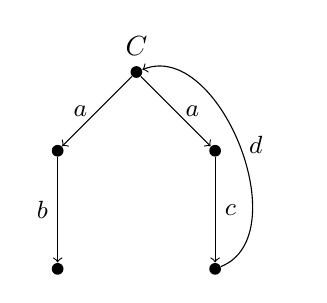
\begin{tikzpicture}[scale=1]

    % Graph nodes
    \node[circle, fill, inner sep=1.5pt, label=above:{$C$}] (0) at (0,0) {};
    \node[circle, fill, inner sep=1.5pt] (a1) at (-1,-1) {};
    \node[circle, fill, inner sep=1.5pt] (a2) at (-1,-2.5) {};
    \node[circle, fill, inner sep=1.5pt] (b1) at (1,-1) {};
    \node[circle, fill, inner sep=1.5pt] (b2) at (1,-2.5) {};

    % Edges with labels
    \draw[->] (0) to node[midway, left] {\small$a$} (a1);
    \draw[->] (0) to node[midway, right] {\small$a$} (b1);
    \draw[->] (a1) to node[midway, left] {\small$b$} (a2);
    \draw[->] (b1) to node[midway, right] {\small$c$} (b2);
    \draw[bend right=90, ->] (b2) to node[midway, right] {\small$d$} (0);

\end{tikzpicture}
 
 \end{center}
\end{example}

